% !TeX spellcheck = cs_CZ
%{\tikzset{external/prefix={tikz/FYZII/}}
% \tikzset{external/figure name/.add={ch27_}{}}
%---------------------------------------------------------------------------------------------------
% file fey2ch27.tex
%---------------------------------------------------------------------------------------------------
%=========================== Kapitola Energie pole a hybnost pole ==================================
\setchaptertoc
\chapter{Energie pole a hybnost pole}\label{fyz:IIchapXXVII}

  \section{Lokální zákony zachování}\label{fyz:IIchapXXVIIsecI}
  \section{Zákon zachování energie a elektromagnetizmus}\label{fyz:IIchapXXVIIsecII}
  \section{Hustota energie a hustota toku energie elektromagnetického 
  pole}\label{fyz:IIchapXXVIIsecIII}
  \section{Nejednoznačnost energie pole}\label{fyz:IIchapXXVIIsecIV}
  \section{Příklady hustoty toku energie}\label{fyz:IIchapXXVIIsecV}
  \section{Hybnost pole}\label{fyz:IIchapXXVIIsecVI}
    \begin{equation}\label{fyz:eq957}
      \vec{g}=\frac{1}{c^2}\,\vec{S}.
    \end{equation}
  \section{Příklady a cvičení}\label{fyz:IIchapXXVIIsecVII}



    \begin{figure}[ht!] %\ref{fyz:fig609}
      \centering
      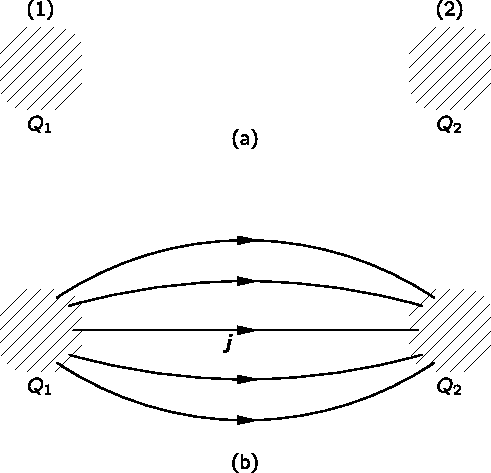
\includegraphics[width=0.7\linewidth]{fyz_fig609.pdf}
      \caption{
               (\cite[s.~707]{Feynman02})}
      \label{fyz:fig609}
    \end{figure}

    \begin{figure}[ht!] %\ref{fyz:fig610}
      \centering
      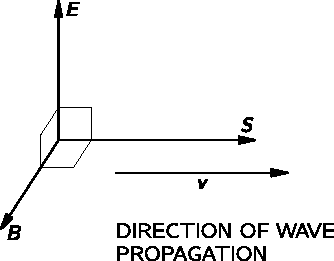
\includegraphics[width=0.7\linewidth]{fyz_fig610.pdf}
      \caption{
               (\cite[s.~707]{Feynman02})}
      \label{fyz:fig610}
    \end{figure}

    \begin{figure}[ht!] %\ref{fyz:fig611}
      \centering
      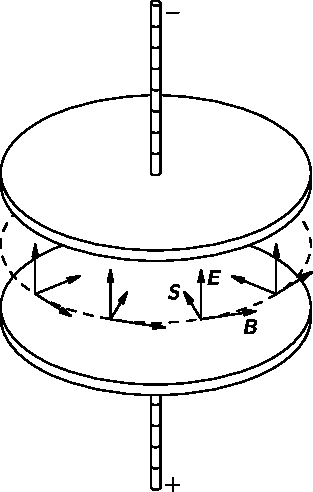
\includegraphics[width=0.7\linewidth]{fyz_fig611.pdf}
      \caption{
               (\cite[s.~707]{Feynman02})}
      \label{fyz:fig611}
    \end{figure}

    \begin{figure}[ht!] %\ref{fyz:fig612}
      \centering
      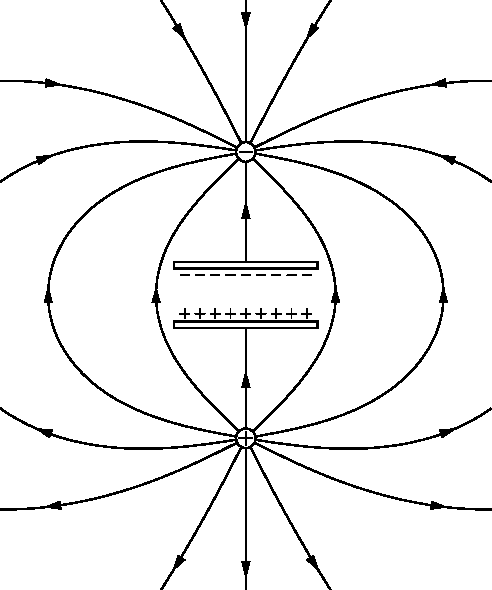
\includegraphics[width=0.7\linewidth]{fyz_fig612.pdf}
      \caption{
               (\cite[s.~707]{Feynman02})}
      \label{fyz:fig612}
    \end{figure}

    \begin{figure}[ht!] %\ref{fyz:fig613}
      \centering
      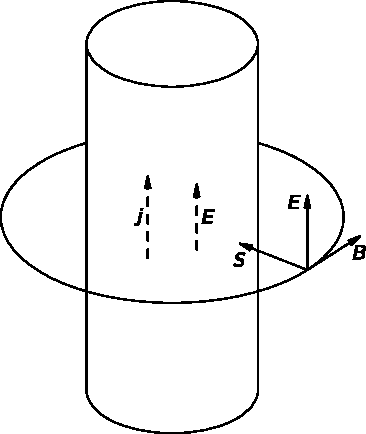
\includegraphics[width=0.7\linewidth]{fyz_fig613.pdf}
      \caption{
               (\cite[s.~707]{Feynman02})}
      \label{fyz:fig613}
    \end{figure}

    \begin{figure}[ht!] %\ref{fyz:fig614}
      \centering
      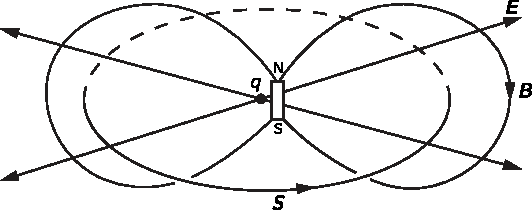
\includegraphics[width=0.7\linewidth]{fyz_fig614.pdf}
      \caption{
               (\cite[s.~707]{Feynman02})}
      \label{fyz:fig614}
    \end{figure}

    \begin{figure}[ht!] %\ref{fyz:fig615}
      \centering
      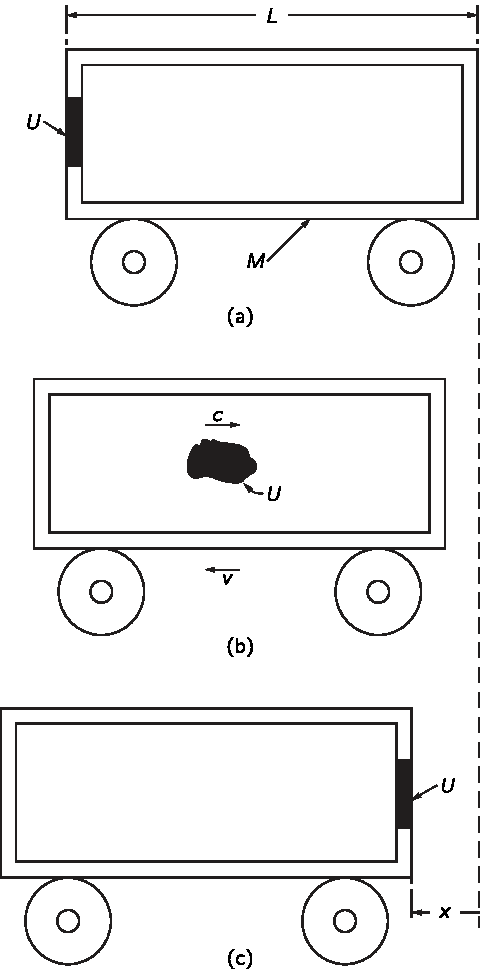
\includegraphics[width=0.7\linewidth]{fyz_fig615.pdf}
      \caption{
               (\cite[s.~707]{Feynman02})}
      \label{fyz:fig615}
    \end{figure}

    \begin{figure}[ht!] %\ref{fyz:fig616}
      \centering
      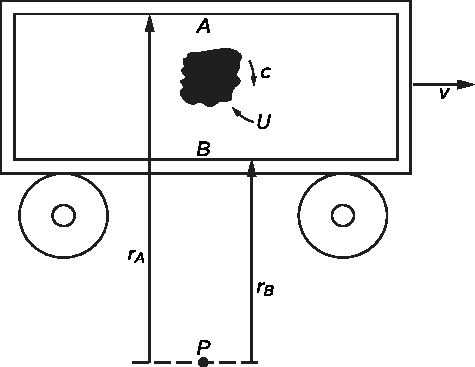
\includegraphics[width=0.7\linewidth]{fyz_fig616.pdf}
      \caption{
               (\cite[s.~707]{Feynman02})}
      \label{fyz:fig616}
    \end{figure}

    \todo[inline]{Kapitola fey2ch27 je nedodělaná, obsahuje pouze obrázky}
%} %tikzset
%---------------------------------------------------------------------------------------------------